\documentclass[titlepage,landscape]{seminar}
\usepackage{url}
\usepackage{graphicx}
\usepackage[pdftex]{color}
\usepackage{hyperref}
\usepackage{epstopdf}
\usepackage{slides}
\usepackage[fleqn]{amsmath}

\begin{document}

\myslide{
\begin{center}
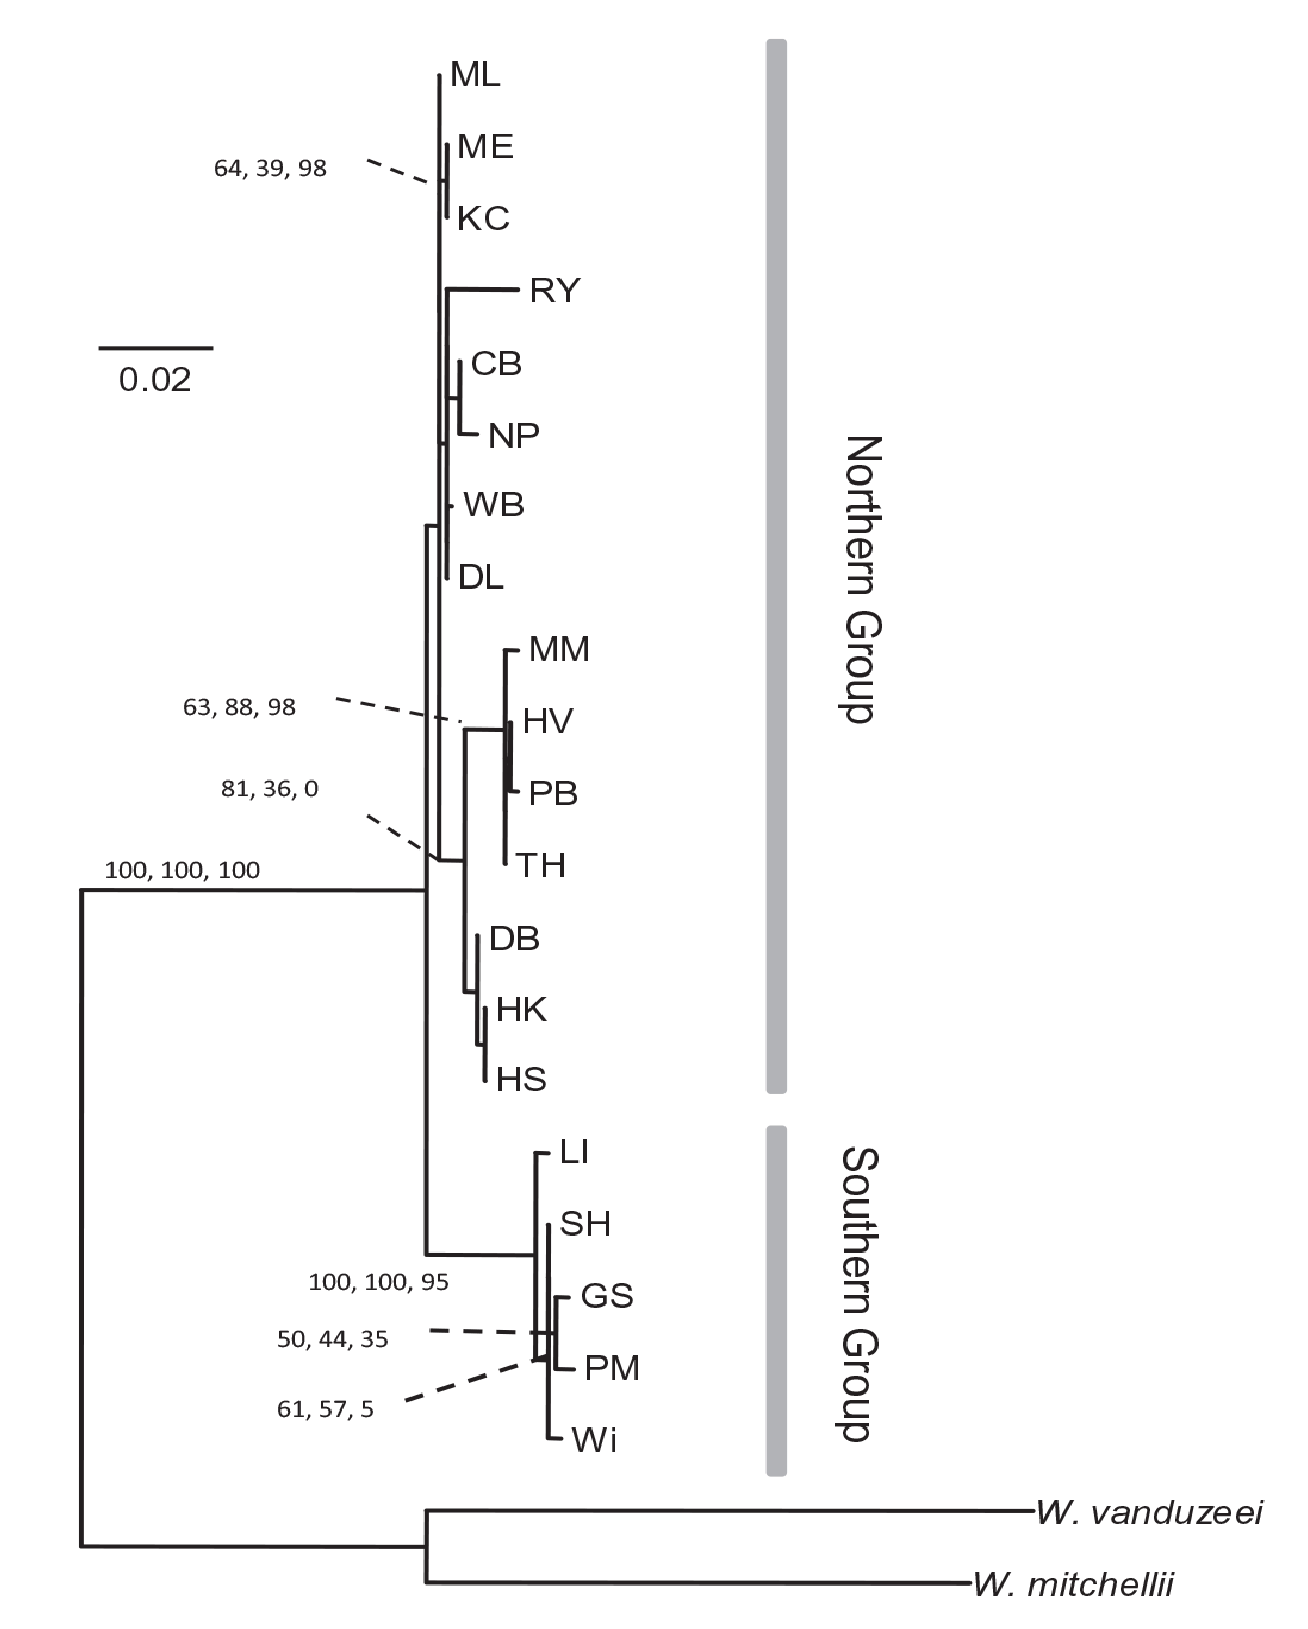
\includegraphics[height=0.9\textheight]{wyeomyia-COI.eps}
\end{center}
}

\myslide{
\begin{center}
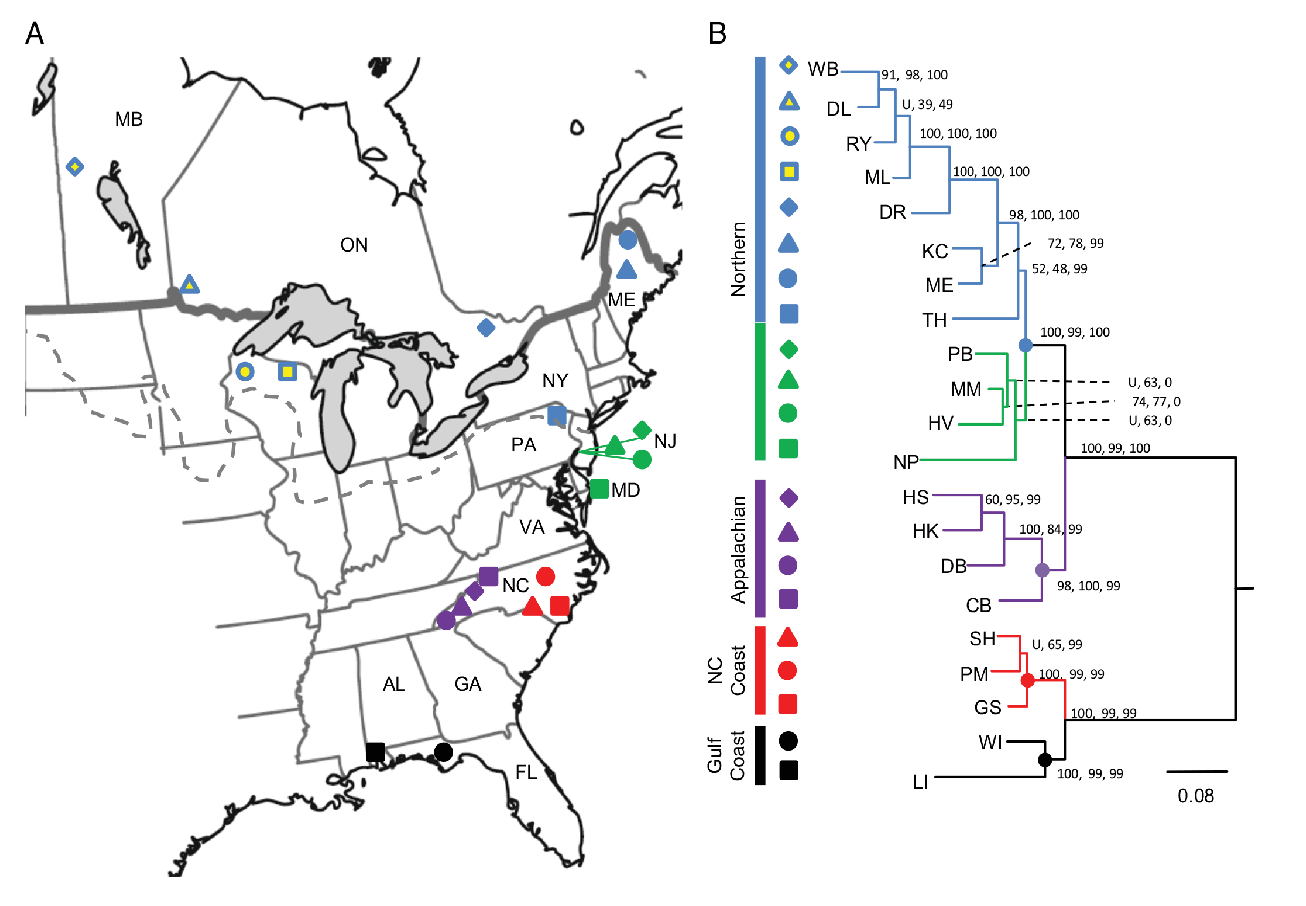
\includegraphics[height=0.9\textheight]{wyeomyia-RAD.eps}
\end{center}
}

\myslide{ 

Interested in estimating $\pi$, the probability that a particular site
is heterozygous

\begin{itemize}

\item site profile: $(n_1, n_2, n_3, n_4)$ number of A, C, G, or T at
  the site

\item $n=n_1+n_2+n_3+n_4$ is the depth of coverage at this site

\item probability of sequencing error: $\epsilon$

\end{itemize}
}

\myslide{
Homozygous site (happens with probability $1-\pi$)
\[
P(n_1,n_2,n_3,n_4|\mbox{homozygous},\epsilon)
=
\sum_{i=1}^4 \left(\frac{p_i^2}{\sum_{j=1}^4p_j^2}\right) 
{n \choose n_i}(1-\epsilon)^{n_i}\epsilon^{n-n_i}
\]
}

\myslide{
Heterozygous site (happens with probability $\pi$)
\begin{eqnarray*}
k_1 &=& \mbox{number of reads from first chromosome} \\
k_2 &=& \mbox{number of reads from second chromosome} \\
P(k_1,k_2) &=& {n \choose k_1}\left(\frac{1}{2}\right)^{k_1}
               \left(\frac{1}{2}\right)^{k_2} \\
&=&
{n \choose k_1}\left(\frac{1}{2}\right)^n
\end{eqnarray*}
}

\myslide{
Ordered genotype $x_ix_j$
{\footnotesize
\[
\begin{aligned}
P(n_1,n_2,n_3,n_4&|x_i,x_j,k_1,k_2) = \\
&\sum_{l=1}^4\sum_{m=0}^{k_1}{k_1 \choose m}(1-\delta_{il})^m\delta_{il}^{k_1-m}
{k_2 \choose n_i-m}(1-\delta_{jl})^{n_1-m}\delta_{jl}^{k_2-(n_1-m)}&&
\end{aligned}
\]
}
\[
\delta_{il} = \left\{\begin{array}{ll}
1-\epsilon & \mbox{if } i = l \\
\epsilon & \mbox{if } i \ne l \quad .
\end{array}
\right.
\]
\[
\begin{aligned}
P(n_1,n_2,n_3,n_4|&x_i,x_j,\epsilon) = \\
&P(n_1,n_2,n_3,n_4|x_i,x_j,k_1,k_2,\epsilon)P(k_1,k_2) \\
P(n_1,n_2,n_3,n_4|&\mbox{heterozygous},\epsilon) = \\
&\sum_{i=1}^4\sum_{j=1}^4
\left(\frac{x_ix_j}{1-{\sum_{l=1}^4p_l^2}}\right) P(n_1,n_2,n_3,n_4|x_i,x_j) 
\end{aligned}
\]
}

\myslide{
\[
\begin{aligned}
P(n_1,n_2,n_3,n_4|\pi,\epsilon)
= 
& \pi P(n_1,n_2,n_3,n_4|\mbox{heterozygous},\epsilon) \\
& +
(1-\pi)P(n_1,n_2,n_3,n_4|\mbox{homozygous},\epsilon)
\end{aligned}
\]
\[
P(\mbox{data}|\pi,\epsilon) = \prod_{s=1}^S
P(n_1^{(s)},n_2^{(s)},n_3^{(s)},n_4^{(s)}|\pi,\epsilon) \quad ,
\]
}

\myslide{
\begin{center}
\begin{tabular}{lccc}
\hline\hline
Taxon & $4N_e\mu$ & $4N_e\mu$ (low coverage) & $\epsilon$ \\
\hline
{\it Cionia intestinalis} & 0.0111 & 0.012 & 0.00113 \\
{\it Daphnia pulex} & 0.0011 & 0.0012 & 0.00121 \\
\hline
\end{tabular}
\end{center}
}

\myslide{ 

316 fully sequenced genes in an African population and a population
with European ancestry.

genome-wide $\Phi_{ST}=0.08$

\begin{itemize}

\item {\bf HSD11B2}: $\Phi_{ST}=0.32 (0.16,0.48)$. Variants at this
  locus are associated with an inherited form of high blood pressure
  and renal disease. A microsatellite in an intron of this locus is
  weakly associated with type 1 diabetes.

\item {\bf FOXA2}: $\Phi_{ST}=0.32 (0.12,0.51)$. This gene is involved
  in reguation of insulin sensitivity.

\item {\bf POLG2}: $\Phi_{ST}=0.33 (0.18,0.48)$. This locus was
  identified as a target of selection in another study.

\end{itemize}

}

\myslide{

12,649 haplotype regions and 11,866 genes derived from 597 individuals
across 33 widely distributed human populations.

$\Phi_{ST}=$ 0.083 (0.075-0.091: chromosome 22) to 0.11 (0.10-0.12:
chromosome 16

\begin{itemize}

\item 569 outliers: 518 ``high''outliers, 51 ``low'' outliers

\item Several ``high'' outliers previously identified as targets of
  selection.

\item None of the ``low'' outliers previously identified as targets of
  selection. Could reflect balancing selection.

\end{itemize}

}

\end{document}


